\chapter{Design of Architecture and Evaluation}
\label{cha:design-and-method}
\epigraph{``Would you tell me, please, which way I ought to go from here?''\\
``That depends a good deal on where you want to get to,'' said the Cat.\\
``I don't much care where—'' said Alice.\\
``Then it doesn't matter which way you go,'' said the Cat.}{\textit{Alice’s Adventures in Wonderland}\\\textsc{Lewis Carroll}}

Many of the other natural sciences have labs with equipment that has to be
configured correctly to experimentally test stated hypotheses.  Such
experiments must be meticulously planned and designed in advance to work
properly and provide valid and trustworthy results.

As computer scientists, we usually do not work in labs, and our experiments
do not live in Petri dishes. Still, we have hypotheses to test, and thus,
experiments to plan. This planning phase is the design of the experiment,
where the authors describe the system intended to test the hypotheses posed
in the introduction.

It is far easier to reason about the design of a system on a whiteboard than
it is to change what has already been committed to code, and it is wise to
carefully consider all aspects of your design, before starting to try to
build it.


\section{Design the System as Well as the Evaluation}
\label{sec:design-system-as}

Some hypotheses can be investigated wholly \emph{in vitro}, testing, \eg one
algorithm against another. Other hypotheses require us to investigate
further, involving, \eg potential users or domain experts to properly
evaluate our assumptions. It is therefore crucial to consider not only
\emph{what} you wish to create, but \emph{how} you propose to evaluate
it. For your study to have validity, the design of the evaluation is every
bit as crucial as the design of the object being evaluated.  How can the
hypotheses described in \autoref{cha:introduction} be investigated?  What is
going to be measured? How will this be accomplished? If the reader is given
a clear plan here, it should also be clear what must be implemented in order
to perform the outlined experiments.  The credibility of your study also
relies on your ability to communicate the process with which you have
reached your design.

\section{Communicating the Design}
\label{sec:communicating-design}


If you have a protocol, or a system that can alternate between several
states in a well-defined manner, a state machine is a very concise way to
communicate this---consider \autoref{fig:profibus} and how much text that
would have required to elucidate.

Another efficient way of communicating systems design is through the use of
\ac{UML} diagrams, both structurally using class diagrams, and behaviourally
using sequence diagrams, see \autoref{fig:WebRTCSignalProcess}, both of
which can be created without any external applications.  These diagrams can
later be referred to, or modified in the next chapter, as there may well be
some differences between your design and your implementation.

\begin{figure}
  \centering
  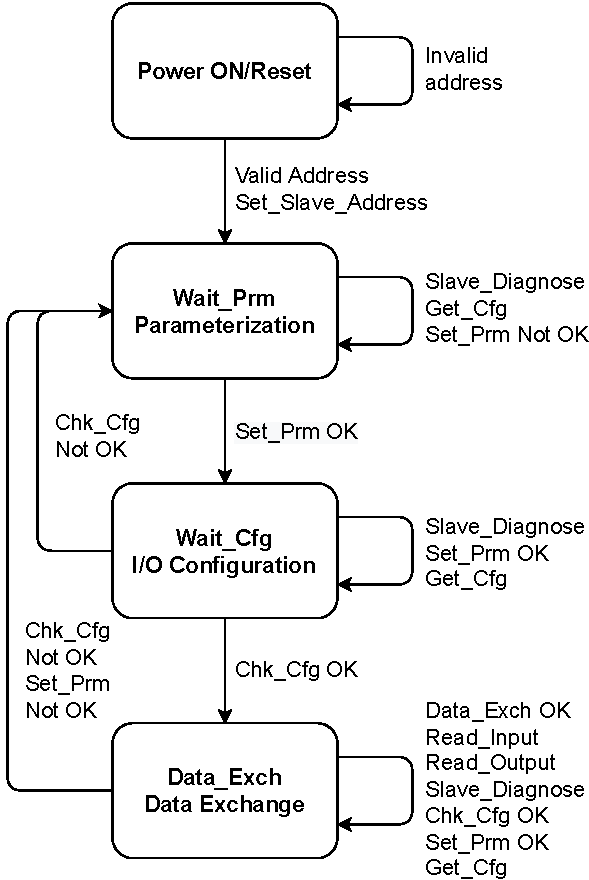
\includegraphics[width=.5\linewidth]{gfx/state_machine_profibus.pdf}
  \caption[Profibus states and transitions]{Profibus states and transitions (\cite{Overgaard2022:2022} used with permission)}
  \label{fig:profibus}
\end{figure}

Indeed, a luxury of this chapter is that the design may well go further than
solely the confirmation or refutation of the hypotheses.  If you are
building a system, this is where you show that you know how to design one,
even if you will actually not be implementing all of it.  If you had
sufficient time and resources, \emph{this} is how you would make your
system.

However, before we come to that, it is necessary to investigate whether the
required hypotheses are valid. If they are not, the design must be
reconsidered, and there is only one way to test them, namely through
implementation, and subsequent evaluation.


%% -----------------------------------------------------------------------------------
%% Created using pgf-umlsd
%% http://mirrors.ibiblio.org/CTAN/graphics/pgf/contrib/pgf-umlsd/pgf-umlsd-manual.pdf
%% -----------------------------------------------------------------------------------
\begin{figure}
  \centering\footnotesize\sffamily
  
    \begin{sequencediagram}
       \newthread{p1}{\normalsize peer 1}
       \newinst[1]{SS}{\normalsize signaling server}
       \newinst[1]{p2}{\normalsize peer 2}
       
       \begin{call}{p1}{getUserMedia()}{p1}{return MediaStream}
       \end{call}
       
       \begin{call}{p1}{addStream()}{p1}{}
       \end{call}

       \begin{call}{p1}{createOffer()}{p1}{}
       \end{call}

       \begin{call}{p1}{setLocalDescription()}{p1}{}
       \end{call}

        
       \begin{messcall}{p1}{send offer}{SS}
            \begin{messcall}{SS}{send offer}{p2}
                \begin{call}{p2}{setRemoteDescription()}{p2}{}
                \end{call}
                \begin{call}{p2}{getUserMedia()}{p2}{}
                \end{call}
                \begin{call}{p2}{addstream()}{p2}{}
                \end{call}
                \begin{call}{p2}{setLocalDescription()}{p2}{}
                \end{call} 
                \begin{messcall}{p2}{send answer}{SS}
                \end{messcall}
            \end{messcall}
            \begin{messcall}{SS}{send answer}{p1}
            \end{messcall}
       \end{messcall}  
      \begin{call}{p1}{setRemoteDescription()}{p1}{}
        \end{call}
       \begin{messcall}{p1}{send ICE candidate}{SS}
            \begin{messcall}{SS}{}{p2}
                \begin{call}{p2}{addIceCandidate()}{p2}{}
                \end{call}
                \begin{messcall}{p2}{send ICE candidate}{SS}
                \end{messcall}
            \end{messcall}
            \begin{messcall}{SS}{send ICE candidate}{p1}
            \end{messcall}
       \end{messcall}
       \begin{call}{p1}{addIceCandidate()}{p1}{}
        \end{call}
    \end{sequencediagram}
    \caption[A sequence diagram example]{A sequence diagram can communinate the interaction between components efficiently (adapted from \cite{Stephansen2017:2017} with permission)}
    \label{fig:WebRTCSignalProcess}
\end{figure}
  
%%% Local Variables:
%%% mode: latex
%%% TeX-master: "../ClassicThesis"
%%% ispell-dictionary: "british" ***
%%% fill-column: 76 ***
%%% End:
